\section{Referencia de la Clase Cliente\-List\-Subform}
\label{classClienteListSubform}\index{ClienteListSubform@{ClienteListSubform}}
Administra el detalle de la lista de clientes.  


{\tt \#include $<$clientslist.h$>$}

Diagrama de herencias de Cliente\-List\-Subform\begin{figure}[H]
\begin{center}
\leavevmode
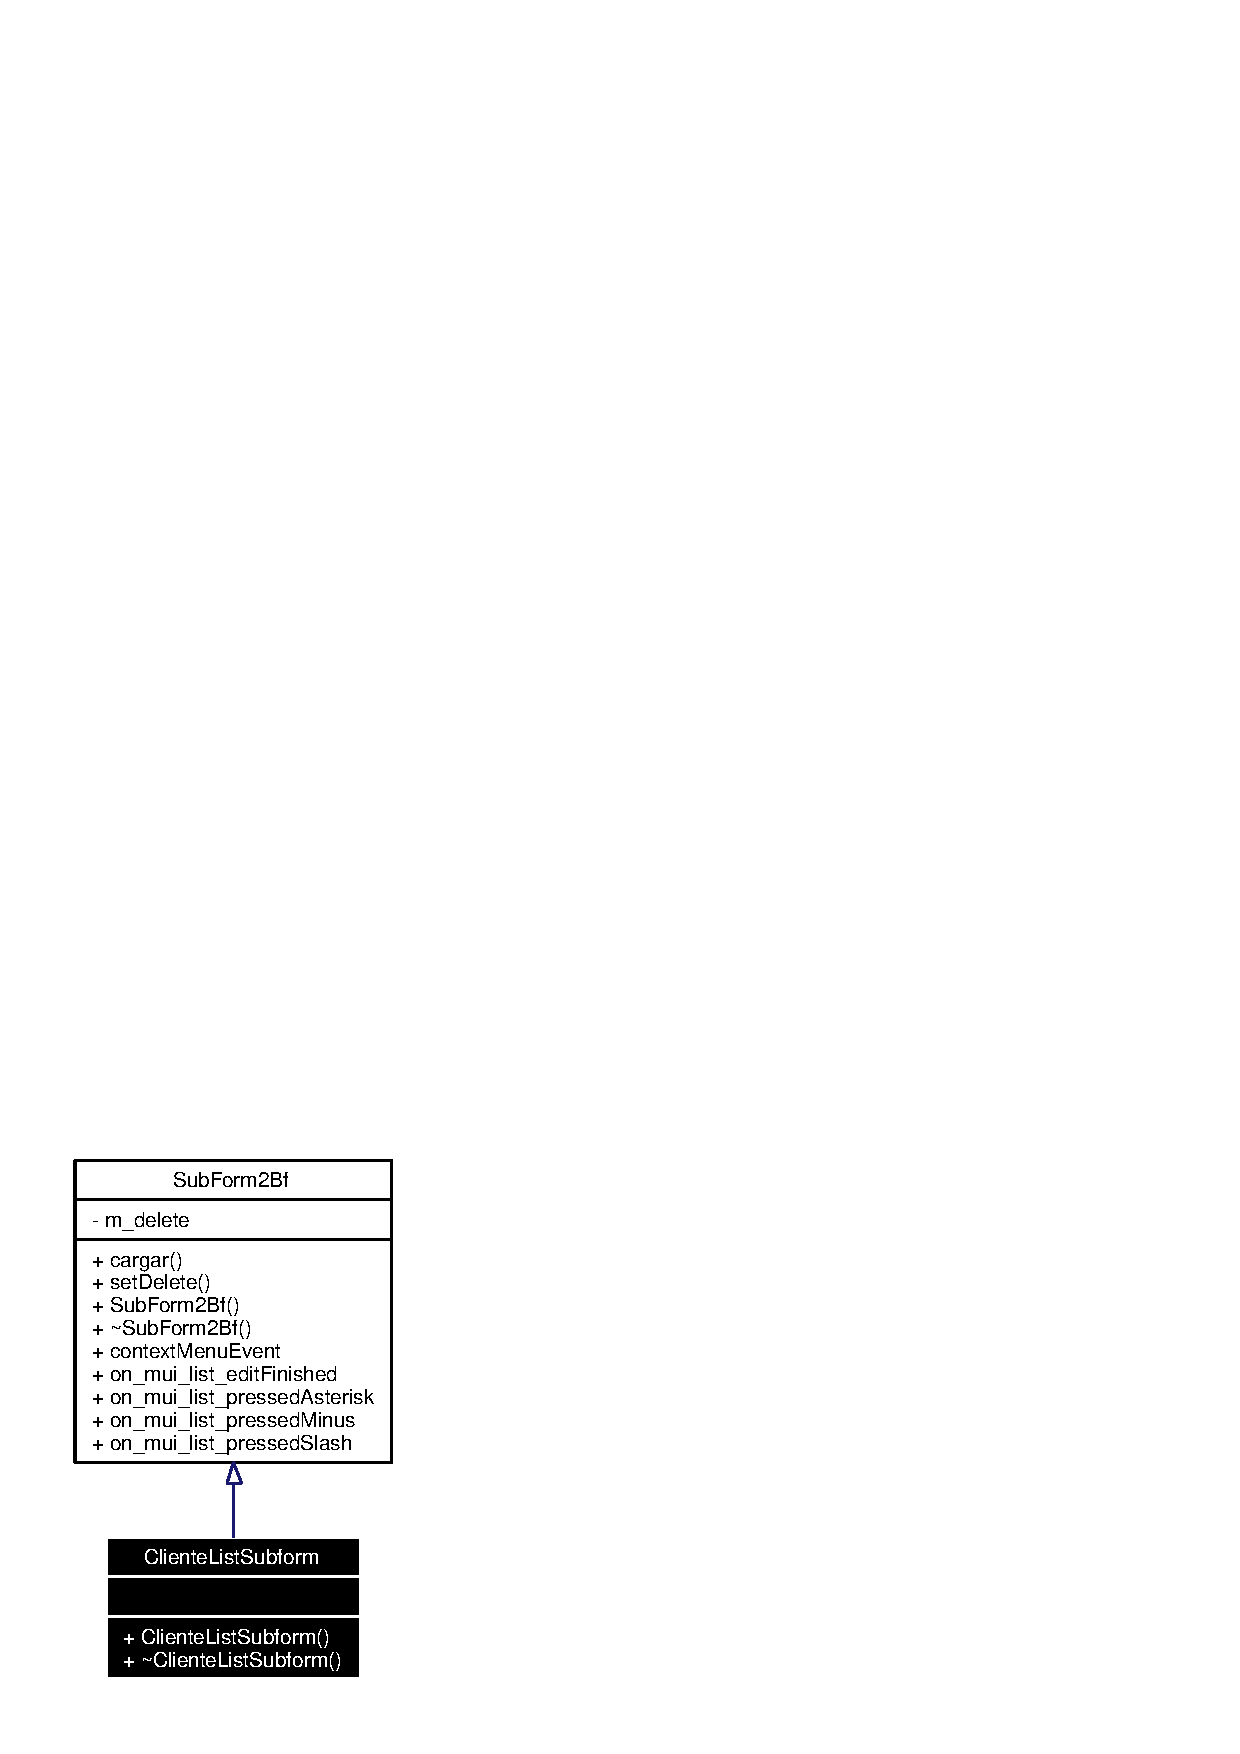
\includegraphics[width=94pt]{classClienteListSubform__inherit__graph}
\end{center}
\end{figure}
Diagrama de colaboraci\'{o}n para Cliente\-List\-Subform:\begin{figure}[H]
\begin{center}
\leavevmode
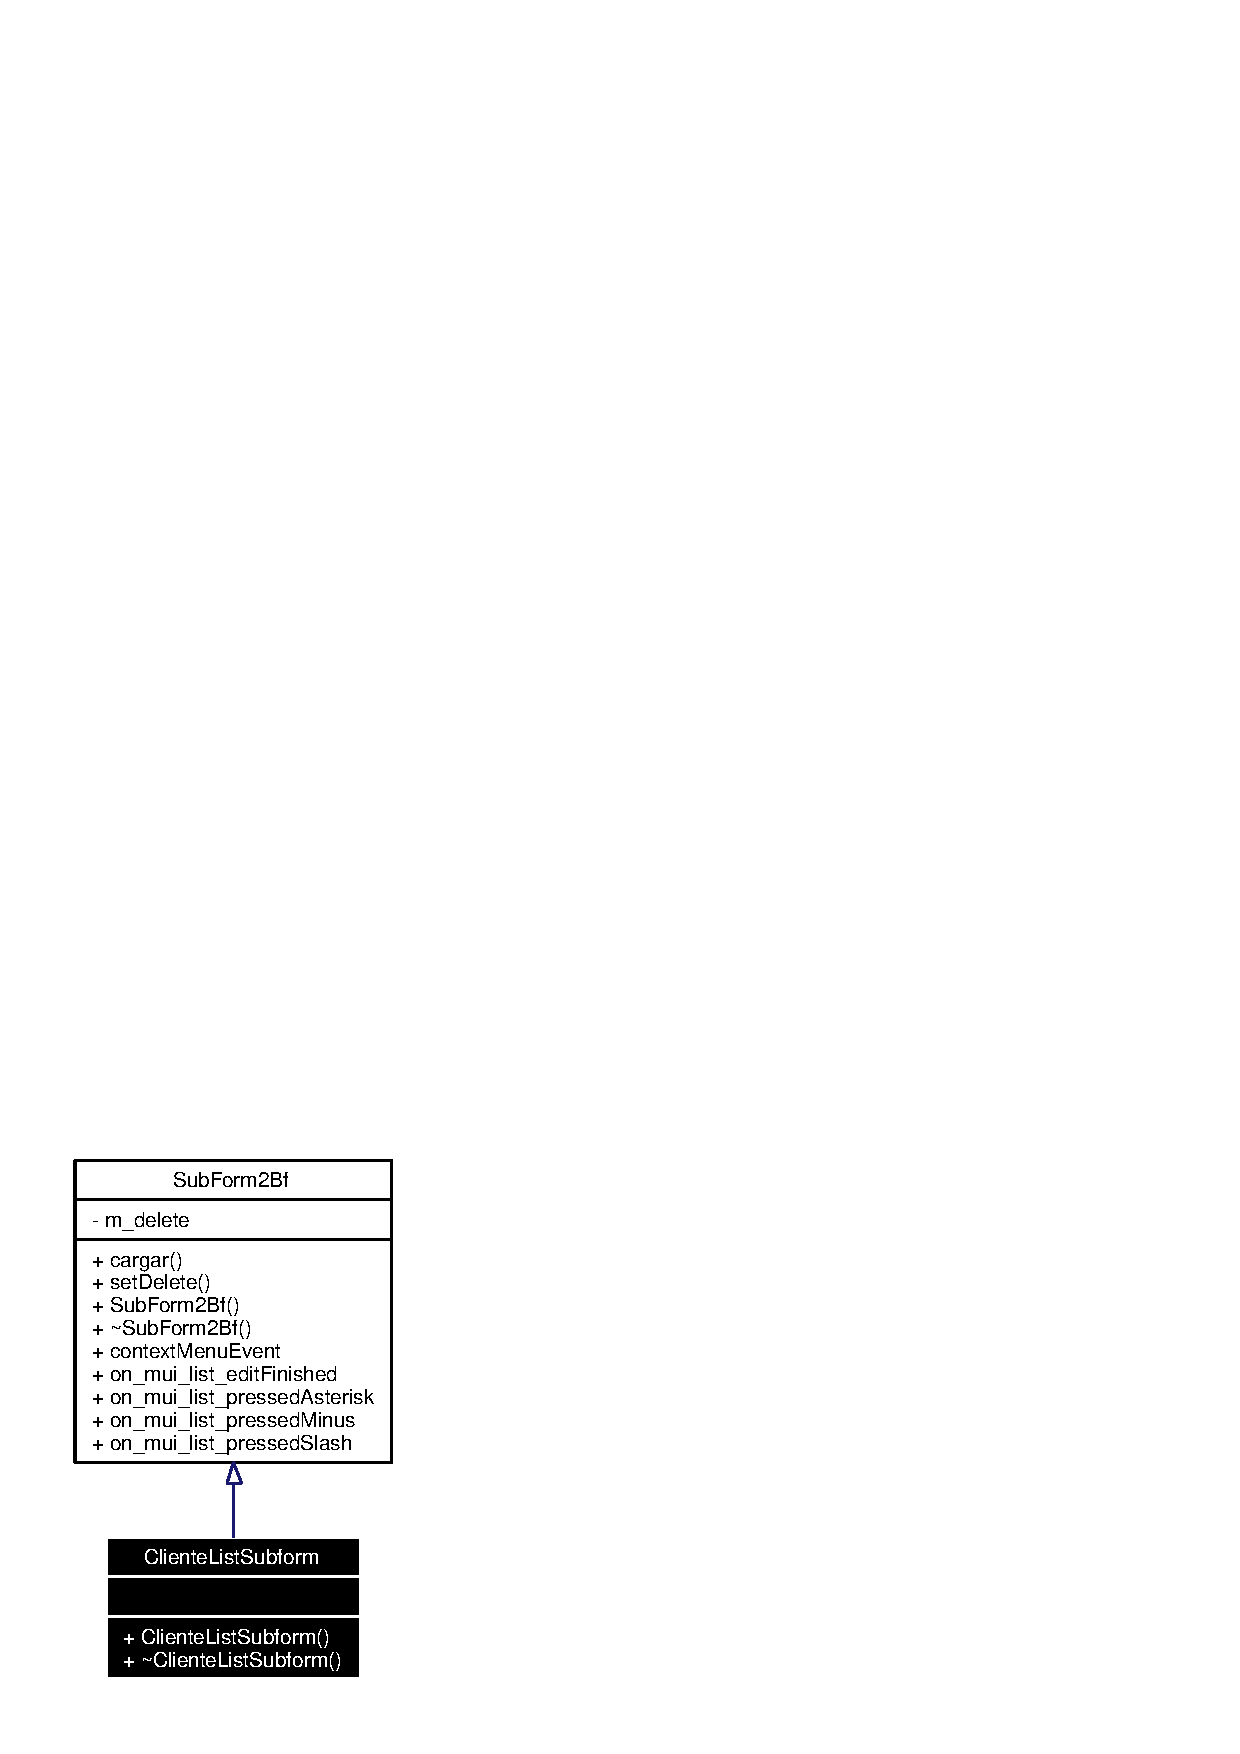
\includegraphics[width=94pt]{classClienteListSubform__coll__graph}
\end{center}
\end{figure}
\subsection*{M\'{e}todos p\'{u}blicos}
\begin{CompactItemize}
\item 
{\bf Cliente\-List\-Subform} (QWidget $\ast$parent=0, const char $\ast$name=0)
\end{CompactItemize}


\subsection{Descripci\'{o}n detallada}
Administra el detalle de la lista de clientes. 



\subsection{Documentaci\'{o}n del constructor y destructor}
\index{ClienteListSubform@{Cliente\-List\-Subform}!ClienteListSubform@{ClienteListSubform}}
\index{ClienteListSubform@{ClienteListSubform}!ClienteListSubform@{Cliente\-List\-Subform}}
\subsubsection{\setlength{\rightskip}{0pt plus 5cm}Cliente\-List\-Subform::Cliente\-List\-Subform (QWidget $\ast$ {\em parent} = {\tt 0}, const char $\ast$ {\em name} = {\tt 0})}\label{classClienteListSubform_a0}


============================================================================= SUBFORMULARIO ============================================================================= 

La documentaci\'{o}n para esta clase fu\'{e} generada a partir de los siguientes archivos:\begin{CompactItemize}
\item 
clientslist.h\item 
clientslist.cpp\end{CompactItemize}
